\documentclass[margin]{res}  

% Default font is the helvetica postscript font
\usepackage{helvet}

% for images adding images
\usepackage{graphics}
\graphicspath{{./}}

% for adding links
\usepackage{hyperref}


% Increase text height
\textheight=700pt

\begin{document}
%-------------------------------------------------------------------------------
%	                    NAME AND ADDRESS SECTION
%-------------------------------------------------------------------------------
\name{Abhinav Lakhani}
\address{
    \\Street No. 2,\\
    Rampara, Jeshingpara,\\
    Amreli, Amreli\\
    Gujarat - 365601
}
\address{\\email-id: \href{3398abhinav@gmail.com}{3398abhinav@gmail.com} \\Contact: (+91) 9586-392952\\
\newline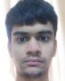
\includegraphics{photo.jpg}}

\begin{resume}

    \section{OBJECTIVE}
    %-------------------------------------------------------------------------------
    %	OBJECTIVE SECTION
    %-------------------------------------------------------------------------------
    {\sl To seek a position in a well established organization that offers room for professional growth, as this provides ample opportunities to learn and use new trends in science \& technologies in industries, while also providing the opportunity to exhibit skills and competencies in my profession for any business I work for.}
    
    \section{EDUCATION}
    %-------------------------------------------------------------------------------
    %	EDUCATION SECTION
    %-------------------------------------------------------------------------------
    \begin{tabular}{||r|c||}
        \hline
        Degree & B. Tech Mechatronics\\
        \hline
        College/school & U. V. Patel College of Engineering (Kherva)\\
        \hline
        University & Ganpat University (Mehsana - Gujarat)\\
        \hline
        Passing Year & 2019\\
        \hline
        Passing Percentage(out of 10) & 6.42 \\
        \hline
    \end{tabular}
    
    \section{PROJECTS}
    %-------------------------------------------------------------------------------
    %	PROJECTS SECTION
    %-------------------------------------------------------------------------------
    \begin{enumerate}
        \item 
    \employer{U. V. P. C. E\\Aug 2018 - April 2019}
    \location{}
    \title{\textbf{Academic Project: Gesture Designated and Voice controlled Robotic Hand using Electro-Myograph Sensor.}}
    \begin{position}
        Worked in a 4 person team to develop an Amazon Alexa controlled desktop based application using python in Raspbian(Raspberry - pi). The application provides an interface to start/initialize the physical robot controlled by raspberry pi. I was responsible for designing the core architecture of the application using python and amazon alexa, as well as performing gesture recognition \& 3D - depth image processing using Xbox 360 Kinect in Matlab via machine learning.
    \begin{itemize}
    \item \textbf{Technology/Tools:} Python, Matlab, Solidworks, Amazon Alexa,\\ 
    Flask(Python), Raspberry-pi, ngrok
    \item \textbf{Link :} \href{https://youtu.be/Pii0wOFBJWE}{https://youtu.be/Pii0wOFBJWE}
    \end{itemize}
    \end{position}
    \end{enumerate}
        
    \section{TRAINING \& \\INTERNSHIP}
    %-------------------------------------------------------------------------------
    %	TRAINING \& \\INTERNSHIP SECTION
    %-------------------------------------------------------------------------------
    \begin{itemize}
        \item \textbf{KALPTARU POWER TRANSMISSION Ltd.\hfill{Jun 18}\\}
                % \normalfont{manufatuuring industry trainee}
        \item \textbf{BOSCH REXROTH\hfill{Jun - July 18}\\}
        \item \textbf{U.V.P.C.E. Ganpat University\hfill{Jun - July 18}}
    \end{itemize}
    \end{resume}

    \section{RESEARCH \\ PUBLICATIONS}
    %-------------------------------------------------------------------------------
    %	RESEARCH \\ PUBLICATIONS SECTION
    %-------------------------------------------------------------------------------
    \begin{enumerate}
        \item none
    \end{enumerate}
  
    \section{TECHNICAL \\ SKILLS}
    %-------------------------------------------------------------------------------
    %	TECHNICAL \\ SKILLS SECTION
    %-------------------------------------------------------------------------------
    \begin{itemize}
    \item \textbf{Languages : } Python, embedded C, C, Matlab 
    \item \textbf{Tools/Framework : } Flask(Python), pyfirmata(Python)
    \item \textbf{Familiar : } Java, Javascript, HTML, CSS, Lua, raspberry-pi  
    \item \textbf{Softwares :} Solidworks, ANSYS, AutoCAD, Matlab \& Simulink, Automation Studio, Keil, Proteus   
    \item \textbf{General : } Electro-Mechanical System design, Robotics, Embedded Systems, Machine Learning, 
                            Data Structures, Algorithm, Object Oriented Programming \\
    \end{itemize}
  
    \section{SOFT \\ SKILLS}
    %-------------------------------------------------------------------------------
    %	SOFT \\ SKILLS SECTION
    %-------------------------------------------------------------------------------
    \begin{enumerate}   
    \item {Hard working }
    \item {Quick learner }
    \item {Ability to perform \& contribute under pressure}
    \item {Flexible \& Adaptable to changes \& challenges}
    \item {Highly Self Motivated}
    \item {Self Confidence \& Positive Attitude}
    \end{enumerate}
  
    \section{EXTRA- \\ CURRICULAR \\ ACTIVITIES}
    %-------------------------------------------------------------------------------
    %	EXTRA- \\ CURRICULAR \\ ACTIVITIES SECTION
    %-------------------------------------------------------------------------------
    \begin{itemize}
    \item \textbf{Tree plantation as well as Garbage removal} at “The Agricultural produce market committee Babra - Amreli(Gujarat)” \hfill{Dec 18}
    \item Organized the Aeromodeling workshop at CONVERGENCE U.V.P.C.E.(2018, National Level Event) \hfill{Feb 18}
    \end{itemize}
  
    \section{CO - \\ CURRICULAR \\ ACTIVITIES}
    %-------------------------------------------------------------------------------
    %	CO- \\ CURRICULAR \\ ACTIVITIES SECTION
    %-------------------------------------------------------------------------------
    \begin{enumerate}   
    \item \textbf{ENGR2000X: A Hands-on Introduction to Engineering Simulations}, a course of study offered by CornellX, an online learning initiative of Cornell University through edX.(VALID CERTIFICATE ID: 863a92cfeaff475aacb63a98dac4e293)
    \item \textbf{Game Development \& Programming: } through online cources.\\ \href{https://github.com/abhinav3398}{https://github.com/abhinav3398}
    \item \textbf{Mechanical System Design: } through online cources.\\ \href{https://grabcad.com/abhinav.lakhani-2}{https://grabcad.com/abhinav.lakhani-2}
    \end{enumerate}
    
\(\)\end{document}